\subsection{$D = \{ a_{1}b_{1}, a_{2}b_{2}, a_{3}b_{3}\}$}\label{subsec:d3c}

In Lemma 14 (ii) of \cite{Sato1}, 
they stated that, when $\sharp \Sigma \geq 3$, for regular patterns $p,q$, if $p\{x:=r\}\preceq q$ for any $r\in D$, then $p\{x:=xy\} \preceq q$ holds, where 
$D = \{ a_{1}b_{1}, a_{2}b_{2}, a_{3}b_{3}\}$ $(a_{i} \ne a_{j} \mbox{ and } b_{i} \ne b_{j} \mbox{ for each } i,j~(i\ne j, 1\le i,j\le 3))$.
Unfortunately, there exist the following counterexamples of Lemma 14 (ii) of \cite{Sato1}.
\begin{ex}\label{CounterExample_Lemma14}
Assume that $a_1=b_2$ and $a_3=b_1$ hold.
  
\begin{itemize}
\item[(1)] 
Let $p=ca_1x^{\prime}a_3c$ and $q=xa_1a_3y$.
It is clear that $\{x:=xy\} \not\preceq q$ holds.
However, we can see that $p\{x^{\prime}:=a_1b_1\}\preceq q$, $p\{x^{\prime}:=a_2b_2\}\preceq q$ and $p\{x^{\prime}:=a_3b_3\}\preceq q$ hold, 
since
$p\{x^{\prime}:=a_1b_1\}=ca_1a_1b_1a_3c=q\{x:=ca_1,y:=a_3c\}$,
$p\{x^{\prime}:=a_2b_2\}=ca_1a_2b_2a_3c=q\{x:=ca_1a_2,y:=c\}$ and 
$p\{x^{\prime}:=a_3b_3\}=ca_1a_3b_3a_3c=q\{x:=c,y:=b_3a_3c\}$ hold.

\item[(2)] 
%Assume that $a_1 = b_2$ and $a_3 = b_1$ hold.
Let $p=cb_2a_1b_1b_2x^{\prime}a_1b_1b_2a_3c$ and $q=xb_2a_1b_1b_2a_3y$.
It is clear that $p\{x:=xy\} \not\preceq q$ holds.
However, we have $p\{x^{\prime}:=a_1b_1\}\preceq q$, $p\{x^{\prime}:=a_2b_2\} \preceq q$, and $p\{x^{\prime}:=a_3b_3\} \preceq q$, 
since  
$p\{x^{\prime}:=a_1b_1\}=cb_2a_1b_1b_2a_1b_1a_1b_1b_2a_3c=q\{x:=cb_2a_1b_1,y:=b_2a_3c\}$,
$p\{x^{\prime}:=a_2b_2\}=cb_2a_1b_1b_2a_2b_2a_1b_1b_2a_3c=q\{x:=cb_2a_1b_1b_2a_2,y:=c\}$,
and  $p\{x^{\prime}:=a_3b_3\}=cb_2a_1b_1b_2a_3b_3a_1b_1b_2a_3c=q\{x:=c,y:=b_3a_1b_1b_2a_3c\}$ hold.
\end{itemize}
\end{ex}

Let $D = \{ a_{1}b_{1}, a_{2}b_{2}, a_{3}b_{3}\}$, where $a_{i} \ne a_{j} \mbox{ and } b_{i} \ne b_{j} \mbox{ for each } i,j~(i\ne j, 1\le i,j\le 3)$.
We consider conditions on $q$ under which satisfies that if $p \{ x := r \} \preceq q$ for all $r \in D$, then $p \{ x := xy \} \preceq q$, where a variable symbol $x$ and $y$ do not appear in $p$ and $q$.
We remark that $a_i$ and $b_j$ may be the same for $i,j (1\le i,j\le 3)$.
Since $p \{ x := r \} \preceq q$ for all $r \in D$ holds, 
there exist the following 10 cases (i)--(xv) for three regular patterns on $\Sigma$ contained in $q$ that correspond to three constant strings in $D$:
Here, $y_1,y_2,y_3$ are variable symbols.

\medskip  

\noindent
\begin{tabular}{ll}
(i)~~~~$a_{1}b_{1}, a_{2}b_{2}, a_{3}b_{3}$ & (vi)~~~$a_{1}b_{1}, y_{1}b_{2}, y_{2}b_{3}$\\
(ii)~~~$a_{1}b_{1}, a_{2}b_{2}, a_{3}y_{1}$ & (vii)~~$y_{1}b_{1}, y_{2}b_{2}, y_{3}b_{3}$\\
(iii)~~$a_{1}b_{1}, a_{2}b_{2}, y_{1}b_{3}$ & (viii)~$y_{1}b_{1}, y_{2}b_{2}, a_{3}y_{3}$\\
(iv)~~~$a_{1}b_{1}, y_{1}b_{2}, a_{3}y_{2}$ & (ix)~~~$y_{1}b_{1}, a_{2}y_{2}, a_{3}y_{3}$\\
(v)~~~~$a_{1}b_{1}, a_{2}y_{1}, a_{3}y_{2}$ & (x)~~~~$a_{1}y_{1}, a_{2}y_{2}, a_{3}y_{3}$
\end{tabular}
\medskip

For cases (v)--(x), it is easy to prove that $p \{ x := xy \} \preceq q$ holds from Lemma \ref{lem:twovariables}.
For example, for case (v), $p \{ x := r \} \preceq q$ for all $r \in \{a_{2}y, a_{3}y\}$ also holds, and therefore $p \{ x := xy \} \preceq q$ holds.
For case (iv), $p \{ x := r \} \preceq q$ for all $r \in \{a_{1}b_{1}, yb_{2}, a_{3}y\}$ also holds.
In order to ensure that $p \{ x := xy \} \preceq q$ holds, the following stronger conditions on $a_{i}$ and $b_{j}$ ($1\le i,j\le 3$) are required, in addition to the conditions $a_{i} \ne a_{j} \mbox{ and } b_{i} \ne b_{j} \mbox{ for all } i,j~(i\ne j, 1\le i,j\le 3)$ derived from Lemmas~\ref{lem:addpart} and \ref{lem:oneside}: $a_{1} \not= b_{2}$ or $b_{1} \not = a_{3}$.
Moreover, since this condition is not symmetric with respect to $a_{i}$ and $b_{i}$ ($1\leq i\leq 3$), it follows that stronger conditions are required overall:
($a_{1} \not= b_{2}$ or $b_{1} \not = a_{3}$) and %for $a_{1}b_{1}, yb_{2}, a_{3}y$.
($a_{1} \not= b_{3}$ or $b_{1} \not = a_{2}$) and %for $a_{1}b_{1}, a_{2}y, yb_{3}$,
($a_{2} \not= b_{3}$ or $b_{2} \not = a_{1}$) and %for $a_{1}y, a_{2}b_{2}, yb_{3}$.
($a_{2} \not= b_{1}$ or $b_{2} \not = a_{3}$) and %for $yb_{1}, a_{2}b_{2}, a_{3}y$,
($a_{3} \not= b_{1}$ or $b_{3} \not = a_{2}$) and %for $yb_{1}, a_{2}y, a_{3}b_{3}$.
($a_{3} \not= b_{2}$ or $b_{3} \not = a_{1}$). %for $a_{1}y, yb_{2}, a_{3}b_{3}$
Therefore, case (iv) will be regarded as the cases in Lemmas~\ref{lem:addpart} and \ref{lem:oneside} instead of $D = \{ a_{1}b_{1}, a_{2}b_{2}, a_{3}b_{3}\}$ for the sake of clarity in the subsequent discussion.
Hence, the subsequent discussion will be restricted to cases (i)--(iii).


The conditions in Lemmas~\ref{lem:3consts_i}, \ref{lem:3consts_ii}, and \ref{lem:3consts_iii} are illustrated in the cases (9), (10), and (11) in Fig.~\ref{fig:lem7bigraph}.

\begin{figure*}[t]
  \begin{center}
    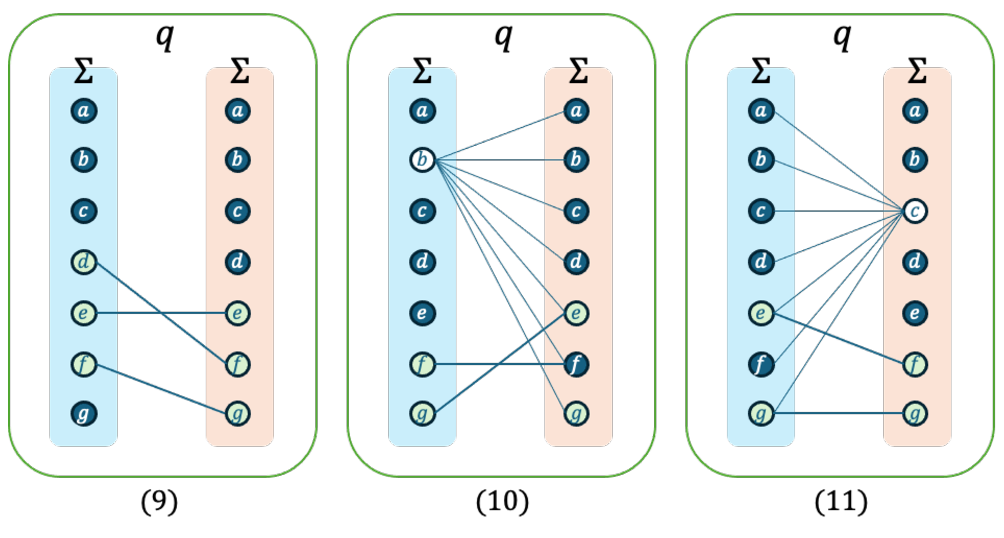
\includegraphics[scale=0.525]{figs/lem7bigraph.pdf}
    \caption{Let $\Sigma=\{a,b,c,d,e,f,g\}$ and $p,q \in \RPat$. We assume that the symbols in $\Sigma$ are mutually distinct.
    The figures (9), (10,) and (11) express cases $D = \{ a_{1}b_{1}, a_{2}b_{2}, a_{3}b_{3} \}$, $D = \{ a_{1}b_{1}, a_{2}b_{2}, a_{3}y \}$, and $D = \{a_{1}b_{1}, a_{2}b_{2}, yb_{3}\}$ in Lemmas~\ref{lem:3consts_i}, \ref{lem:3consts_ii}, and \ref{lem:3consts_iii}, respectively, where $a_{i} \ne a_{j} \mbox{ and } b_{i} \ne b_{j} \mbox{ for each } i,j~(i\ne j, 1\le i,j\le 3)$.
    In these cases, if $p \{ x := r \} \preceq q$ for all $r \in D$, then $p \{ x := xy \} \preceq q$ holds.}\label{fig:lem7bigraph}
  \end{center}
\end{figure*}

%\medskip
%\noindent
\begin{lem}\label{lem:3consts_i}
Let $D = \{ a_{1}b_{1}, a_{2}b_{2}, a_{3}b_{3}\}$, where $a_{i} \ne a_{j} \mbox{ and } b_{i} \ne b_{j} \mbox{ for each } i,j~(i\ne j, 1\le i,j\le 3)$.
Let $p = p_{1}xp_{2}$ for $p_{1},p_{2} \in \RPat \cup \{\varepsilon\}$ and $x \in X$.
If for all $r \in D$, there exist $q_{r,1}$ and $q_{r,2} \in \RPat \cup \{\varepsilon\}$ such that
\begin{enumerate}
\item[1.] $p_{i} \preceq q_{r,i}$ $(i=1,2$) and
\item[2.] $p_{1}rp_{2} \preceq q_{r,1}rq_{r,2}$,
\end{enumerate}
then $p \{ x := xy \} \preceq q$ holds.  
\end{lem}

\begin{proof}
%(I) Case of (i), that are the cases that $q$ contains $a_{1}b_{1}, a_{2}b_{2}$ and $a_{3}b_{3}$:
%\begin{figure}
%\centering
%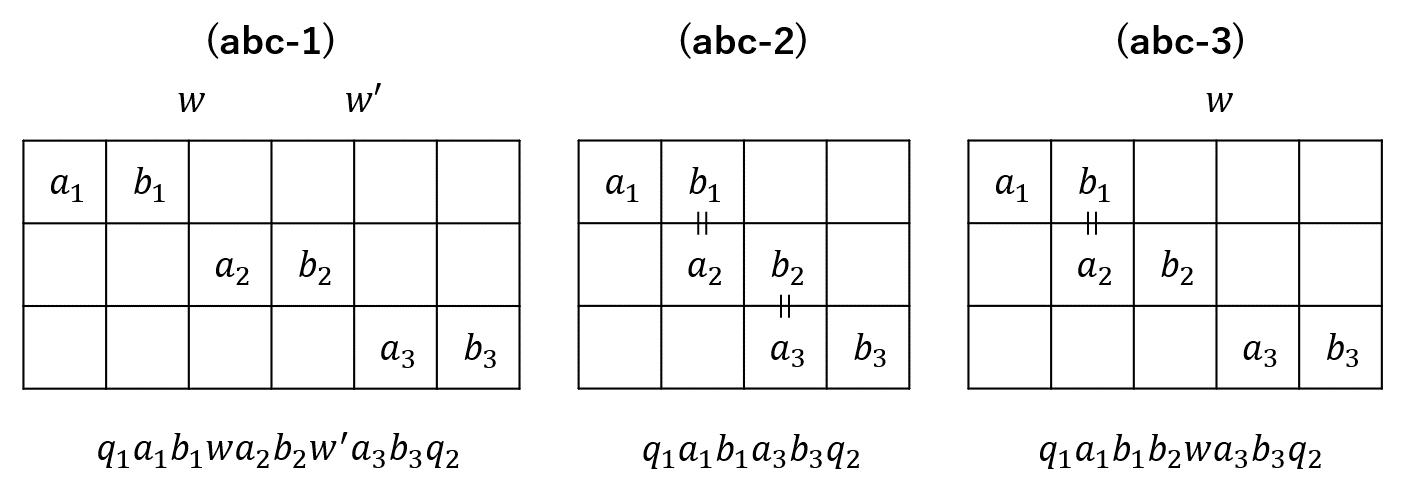
\includegraphics[width=\linewidth]{figs/Cases-abc.png}
%\vspace{-1cm}
%\caption{(abc)の場合分け}
%\label{abc組み合わせ}
%\end{figure}
%\noindent
This corresponds to case (i).
We assume that $p \{ x := xy \} \not\preceq q$ holds. 
We consider the following four cases (I-1)-(I-4) of $q$ for some regular patterns $q_{1},q_{2}$ and some constant strings $w,w^{\prime}$ ($|w|\geq 0$ and $|w^{\prime}|\geq 0$):

\smallskip
\noindent
\begin{tabular}{ll}
(I-1) $q=q_{1}a_{1}b_{1}wa_{2}b_{2}w^{\prime}a_{3}b_{3}q_{2}$,\\
(I-2) $q=q_{1}a_{1}b_{1}a_{3}b_{3}q_{2}$ ($b_{1}=a_{2}$ and $a_{3}=b_{2}$),\\
(I-3) $q=q_{1}a_{1}b_{1}b_{2}wa_{3}b_{3}q_{2}$ ($b_{1}=a_{2}$),\\
(I-4) $q=q_{1}a_{1}b_{1}wa_{2}b_{2}b_{3}q_{2}$ ($b_{2}=a_{3}$).
\end{tabular}
\smallskip

\noindent
(I-1) Case of $q=q_{1}a_{1}b_{1}wa_{2}b_{2}w^{\prime}a_{3}b_{3}q_{2}$:
Assume that the following six conditions (1),(2),(3),(1'),(2'),(3') are hold.
\begin{align*}
\textrm{(1)}~& p_{1} \preceq q_{1} & \textrm{(1')}~& p_{2} \preceq wa_{2}b_{2}w^{\prime}a_{3}b_{3}q_{2} \\
\textrm{(2)}~& p_{1} \preceq q_{1}a_{1}b_{1}w & \textrm{(2')}~& p_{2} \preceq w^{\prime}a_{3}b_{3}q_{2} \\
\textrm{(3)}~& p_{1} \preceq q_{1}a_{1}b_{1}wa_{2}b_{2}w^{\prime} & \textrm{(3')}~& p_{2} \preceq q_{2}
\end{align*}

If $|w|=|w^{\prime}|$ holds, $a_{1}b_{1}wa_{2}b_{2}w^{\prime}$ and $a_{1}b_{1}w$ are the suffix of $p_{1}$ from the above conditions (2) and (3).
Then, $a_{1}b_{1}w=a_{2}b_{2}w^{\prime}$.
Hence, $a_{1}b_{1}=a_{2}b_{2}$.
This contracts the assumption of $a_{1} \ne a_{2}$ and $b_{1} \ne b_{2}$.

If $|w|+1=|w^{\prime}|$ holds, $wa_{2}b_{2}w^{\prime}a_{3}b_{3}$ and $w^{\prime}a_{3}b_{3}$ are the prefix of $p_{2}$.
If there exists a constant symbol $w_{1}$ such that $w^{\prime}a_{3}b_{3}=ww_{1}a_{3}b_{3}$,
then $b_{2}$ and $a_{3}$ are the same symbol from $wa_{2}b_{2}=ww_{1}a_{3}$.
From the above conditions (2) and (3), $a_{1}b_{1}wa_{2}b_{2}w^{\prime}$ and $a_{1}b_{1}w$ are the suffix of $p_{1}$.
Then, there exists a constant symbol $w_{2}$ such that $w^{\prime}=w_{2}w$,
then $b_{2}$ and $a_{1}$ are the same symbol from $b_{2}w_{2}w=a_{1}b_{1}w$.
Hence, from $b_{2}=a_{3}$, $a_{3}$ and $a_{1}$ are same symbol.
This contradicts the assumption of $a_{3} \ne a_{1}$.

If $|w|+1 < |w^{\prime}|$, from the above (2) and (3), 
$a_{1}b_{1}wa_{2}b_{2}w^{\prime}$ and $a_{1}b_{1}w$ are the suffix of $p_{1}$.
If there exists a constant string $w_{1}$ ($|w_{1}|\geq 2$) such that $w^{\prime}=w_{1}w$, then $a_{1}b_{1}$ is the suffix of $w_{1}$.
From  the above conditions ($1'$) and ($2'$), 
$wa_{2}b_{2}w^{\prime}a_{3}b_{3}$ and $w^{\prime}a_{3}b_{3}$ are the prefix of $p_{2}$.
If there exist constant strings $w_{1}$ and $w_{2}$ such that $w^{\prime} = w_{1}w=ww_{2}$ holds, then $a_{2}b_{2}$ and $a_{3}b_{3}$ are the suffix of $w_{1}$ from $|w_1|=|w_2|$ and $|ww_{2}a_{3}b_{3}|=|wa_{2}b_{2}w_{1}|$.
Hence, $a_{1}b_{1}=a_{3}b_{3}$.
This contradicts the assumption of $a_{1} \ne a_{3}$ and $b_{1} \ne b_{3}$.
%\smallskip

If $|w|>|w^{\prime}|$, we can prove the contradiction in a similar way as $|w|\le|w^{\prime}|$.

\smallskip

\noindent
(I-2) Case of $q=q_{1}a_{1}b_{1}a_{3}b_{3}q_{2}$ ($b_{1}=a_{2}$ and $a_{3}=b_{2}$):
Assume that the following six conditions (1),(2),(3),(1'),(2'),(3') are hold.
\begin{align*}
\textrm{(1)}~& p_{1} \preceq q_{1} & \textrm{(1')}~& p_{2} \preceq a_{3}b_{3}q_{2} \\
\textrm{(2)}~& p_{1} \preceq q_{1}a_{1} & \textrm{(2')}~& p_{2} \preceq b_{3}q_{2} \\
\textrm{(3)}~& p_{1} \preceq q_{1}a_{1}b_{1} & \textrm{(3')}~& p_{2} \preceq q_{2}
\end{align*}

\noindent
From the above conditions (2) and (3), since $a_{1}b_{1}$ and $a_{1}$ are the suffix of $p_{1}$, 
$b_{1} = a_{1}$ holds.
From the assumption of $b_{1}=a_{2}$, $a_{1}=a_{2}$.
This contradicts the assumption of $a_{1}\not= a_{2}$.
\smallskip

\noindent
(I-3) Case of $q=q_{1}a_{1}b_{1}b_{2}wa_{3}b_{3}q_{2}$ ($b_{1}=a_{2}$):
Assume that the following six conditions (1),(2),(3),(1'),(2'),(3') are hold.
\begin{align*}
\textrm{(1)}~& p_{1} \preceq q_{1} & \textrm{(1')}~& p_{2} \preceq b_{2}wa_{3}b_{3}q_{2} \\
\textrm{(2)}~& p_{1} \preceq q_{1}a_{1} & \textrm{(2')}~& p_{2} \preceq wa_{3}b_{3}q_{2} \\
\textrm{(3)}~& p_{1} \preceq q_{1}a_{1}b_{1}b_{2}w & \textrm{(3')}~& p_{2} \preceq q_{2}
\end{align*}

%\noindent
If $|w|=0$, i.e., $w$ is the empty string, then $a_{1}$ and $a_{1}b_{1}b_{2}$ are the suffix of $p_{1}$ from the above conditions (2) and (3)
and $b_{2}a_{3}b_{3}$ and $a_{3}b_{3}$ are the prefix of $p_{2}$ from the above conditions (1') and (2').
Since $b_{2}=a_{1}$ and $b_{2}a_{3}=a_{3}b_{3}$, $a_{1}=a_{3}$ holds.
This contradicts the assumption of $a_{1}\not= a_{3}$.

%\noindent
If $|w| \ge 1$, $a_{1}$ and $a_{1}b_{1}b_{2}w$ are the suffix of $p_{1}$ from the above conditions (2) and (3).
Hence, the last symbol of $w$ is $a_{1}$.
Moreover, $b_{2}wa_{3}b_{3}$ and $wa_{3}b_{3}$ are the prefix of $p_{2}$ from the above conditions (1') and (2').
Hence, the last symbol of $w$ is $a_{3}$.
Therefore, $a_{1}=a_{3}$ holds.
This contradicts the assumption of $a_{1} \ne a_{3}$.
\smallskip

\noindent
(I-4) Case of $q=q_{1}a_{1}b_{1}wa_{2}b_{2}b_{3}q_{2}$ ($b_{2}=a_{3}$):
Assume that the following six conditions (1),(2),(3),(1'),(2'),(3') are hold.
\begin{align*}
\textrm{(1)}~& p_{1} \preceq q_{1} & \textrm{(1')}~& p_{2} \preceq wa_{2}b_{2}b_{3}q_{2} \\
\textrm{(2)}~& p_{1} \preceq q_{1}a_{1}b_{1}w & \textrm{(2')}~& p_{2} \preceq b_{3}q_{2} \\
\textrm{(3)}~& p_{1} \preceq q_{1}a_{1}b_{1}wa_{2} & \textrm{(3')}~& p_{2} \preceq q_{2}
\end{align*}
\noindent

%\noindent
If $|w|=0$, i.e., $w$ is the empty string, then $a_{1}b_{1}$ and $a_{1}b_{1}a_{2}$ are the suffix of $p_{1}$ from the above conditions (2) and (3)
and $a_{2}b_{2}b_{3}$ and $b_{3}$ are the prefix of $p_{2}$ from the above conditions (1') and (2').
Since $b_{1}=a_{2}$ and $a_{2}=b_{3}$, then $b_{1}=b_{3}$ holds.
This contradicts the assumption of $b_{1}\not= b_{3}$.

%\noindent
If $|w| \ge 1$, since $a_{1}b_{1}w$ and $a_{1}b_{1}wa_{2}$ are the suffix of $p_{1}$ from the above conditions (2) and (3), the first symbol of $w$ is $b_{1}$.
Moreover, since $wa_{2}b_{2}b_{3}$ and $b_{3}$ are the prefix of $p_{2}$ from the above conditions (1') and (2'),
the first symbol of $w$ is $b_{3}$.
Therefore, $b_{1}=b_{3}$ holds.
This contradicts the assumption of $b_{1} \ne b_{3}$.
\end{proof}

\begin{lem}\label{lem:3consts_ii}
  Let $D = \{ a_{1}b_{1}, a_{2}b_{2}, a_{3}b_{3}\}$, where $a_{i} \ne a_{j} \mbox{ and } b_{i} \ne b_{j} \mbox{ for each } i,j~(i\ne j, 1\le i,j\le 3)$.
  Let $p = p_{1}x_{2}$ for $p_{1},p_{2} \in \RPat \cup \{\varepsilon\}$ and $x \in X$.
  If for all $r \in D$, there exist $q_{r,1}$ and $q_{r,2} \in \RPat \cup \{\varepsilon\}$ such that 
  \begin{enumerate}
  \item[1.] $p_{1} \preceq q_{r,1}$,
  \item[2.] $p_{2} \preceq q_{r,2}$ if $r \in \{a_{1}b_{1}, a_{2}b_{2}\}$,
  \item[3.] $p_{2} \preceq q_{r,2}$ or $p_{2} \preceq y_{1}^{\prime}q_{r,2}$ if $r = a_{3}b_{3}$ ($y_{1}^{\prime} \in X$),
  \item[4.] $p_{1}rp_{2} \preceq q_{r,1}rq_{r,2}$ if $r \in \{a_{1}b_{1}, a_{2}b_{2}\}$, and
  \item[5.] $p_{1}rp_{2} \preceq q_{r,1}a_{3}y_{1}q_{r,2}$ if $r = a_{3}b_{3}$ ($y_{1} \in X)$,
  \end{enumerate}
then $p \{ x := xy \} \preceq q$ holds.  
\end{lem}

\begin{proof}
This corresponds to case (ii).
We assume that $p \{ x := xy \} \not\preceq q$ holds. 
Let $A,B,C$ be distinct regular patterns in $\{a_{1}b_{1}, a_{2}b_{2}, a_{3}y\}$ such that $q=q_{1}AwBw^{\prime}Cq_{2}$.
Assume that the following six conditions (1),(2),(3),(1'),(2'),(3') are hold.
\begin{align*}
\textrm{(1)}~& p_{1} \preceq q_{1} & \textrm{(1')}~& p_{2} \preceq wBw^{\prime}Cq_{2} \\
\textrm{(2)}~& p_{1} \preceq q_{1}Aw & \textrm{(2')}~& p_{2} \preceq w^{\prime}Cq_{2} \\
\textrm{(3)}~& p_{1} \preceq q_{1}AwBw^{\prime} & \textrm{(3')}~& p_{2} \preceq q_{2}
\end{align*}

%\noindent
If $|w|=|w^{\prime}|$, then $Aw$ and $AwBw^{\prime}$ are the suffix of $p_{1}$ from the above conditions (2) and (3).
Hence, $Aw=Bw^{\prime}$ holds.
This contradicts the assumption of $A \ne B$.

%\noindent
If $|w| \ne |w^{\prime}|$, then we consider the two cases $A=a_{3}y$ and $B=a_{3}y$:
In the case of $A=a_{3}y$, without losing generality, we assume that $B=a_{1}b_{1}$ and $C=a_{2}b_{2}$. 
Then, there exist regular patterns $p_{1}^{\prime}, p_{1}^{\prime\prime}$ such that $p_{1}=p_{1}^{\prime}p_{1}^{\prime\prime}$, $p_{1}^{\prime} \preceq q_{1}a_{3}$ and $p_{1}^{\prime\prime} \preceq yw$ from the above condition (2).
Moreover, from the above condition (1'), $p=p_{1}xp_{2}=p_{1}^{\prime}p_{1}^{\prime\prime}xp_{2}\preceq q_{1}a_{3}p_{1}^{\prime\prime}xwa_{1}b_{1}w^{\prime}a_{2}b_{2}q_{2}=
q_{1}a_{3}ywa_{1}b_{1}w^{\prime}a_{2}b_{2}q_{2}\{ y := p_{1}^{\prime\prime}x \}=q \{ y := p_{1}^{\prime\prime}x \}$ holds.
Hence, $p \preceq q$ holds.
This contracts the assumption.
In the case of $B=a_{3}y$, without losing generality, we assume that $A=a_{1}b_{1}$ and $C=a_{2}b_{2}$.
Let $q_{1}^{\prime}=q_{1}a_{1}b_{1}$, $q_{2}^{\prime}=wa_{3}yw^{\prime}$, and $q_{3}^{\prime}=a_{2}b_{2}q_{2}$ such that $q_{2}^{\prime}$ contains at most one variable symbol.
Then, the above conditions (3) and (1') are represented by $p_{1} \preceq q_{1}^{\prime}q_{2}^{\prime}$ and $p_{2} \preceq q_{2}^{\prime}q_{3}^{\prime}$, respectively.
From Theorem \ref{Sato1:Lemma9}, $p \preceq q$ holds.
This contradicts the assumption.

%\begin{figure}
%  \centering
%  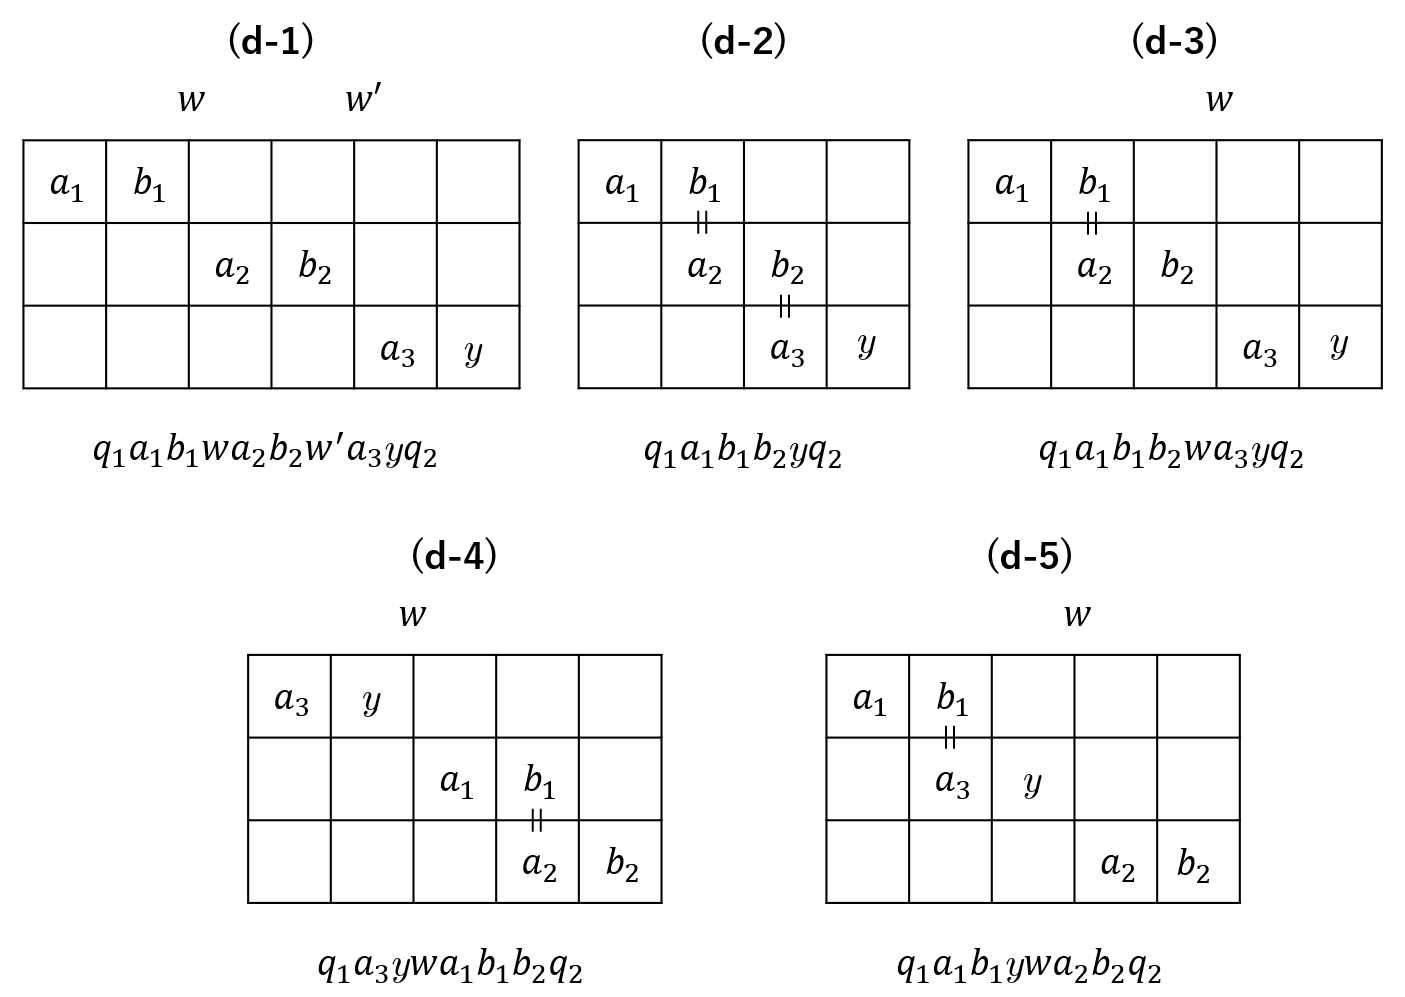
\includegraphics[width=\linewidth]{figs/Cases-d.png}
%  \vspace{-1cm}
%  \caption{(d)の場合分け}
%  \label{d組み合わせ}
%\end{figure}
    
Next, in the case of $C=a_{3}y$, we consider the following five cases (II-1)--(II-5):

\begin{tabular}{l}
(II-1) $q=q_{1}a_{1}b_{1}wa_{2}b_{2}w^{\prime}a_{3}yq_{2}$,\\
(II-2) $q=q_{1}a_{1}b_{1}b_{2}yq_{2}$ ($a_{2}=b_{1}$ and $a_{3}=b_{2}$),\\
(II-3) $q=q_{1}a_{1}b_{1}b_{2}wa_{3}yq_{2}$ ($b_{1}=a_{2}$),\\
(II-4) $q=q_{1}a_{3}ywa_{1}b_{1}b_{2}q_{2}$ ($b_{1}=a_{2}$),\\
(II-5) $q=q_{1}a_{1}b_{1}ywa_{2}b_{2}q_{2}$ ($b_{1}=a_{3}$).
\end{tabular}

\smallskip
\noindent
(II-1) Case of $q=q_{1}a_{1}b_{1}wa_{2}b_{2}w^{\prime}a_{3}yq_{2}$:
Assume that the following six conditions (1),(2),(3),(1'),(2'),(3') are hold.
\begin{align*}
\textrm{(1)}~& p_{1} \preceq q_{1} & \textrm{(1')}~& p_{2} \preceq wa_{2}b_{2}w^{\prime}a_{3}yq_{2} \\
\textrm{(2)}~& p_{1} \preceq q_{1}a_{1}b_{1}w & \textrm{(2')}~& p_{2} \preceq w^{\prime}a_{3}yq_{2} \\
\textrm{(3)}~& p_{1} \preceq q_{1}a_{1}b_{1}wa_{2}b_{2}w^{\prime} & \textrm{(3')}~& p_{2} \preceq q_{2}
\end{align*}

%\noindent
If $|w|+1=|w^{\prime}|$, then $a_{1}b_{1}wa_{2}b_{2}w^{\prime}$ and $a_{1}b_{1}w$ are the suffix of $p_{1}$ from the above conditions (2) and (3).
Since there exists a constant symbol $w_{1}$ such that $w^{\prime}=w_{1}w$ and $b_{2}w_{1}w=a_{1}b_{1}w$ hold,
then $b_{2}=a_{1}$.
Moreover, $wa_{2}b_{2}w^{\prime}a_{3}$ and $w^{\prime}a_{3}$ are the prefix of $p_{2}$ from the above conditions (1') and (2').
Since there exists a constant symbol $w_{2}$ such that $w^{\prime}=ww_{2}$ and $wa_{2}b_{2}=ww_{2}a_{3}$ hold,
then $b_{2}=a_{3}$.
Thus, $a_{1} = a_{3}$ holds.
This contradicts the assumption of $a_{1} \ne a_{3}$.

%\noindent
If $|w|+1 < |w^{\prime}|$, then $a_{1}b_{1}wa_{2}b_{2}w^{\prime}$ and $a_{1}b_{1}w$ are the suffix of $p_{1}$ from the above conditions (2) and (3).
Hence, $a_{1}b_{1}$ is the suffix of $w_{\prime}$.
Moreover, $wa_{2}b_{2}w^{\prime}a_{3}$ and $w^{\prime}a_{3}$ are the prefix of $p_{2}$ from the above conditions (1') and (2').
Hence, there exist constant symbols $w_{1}$ and $w_{2}$ such that $w^{\prime}=w_{1}w$, $w^{\prime}=ww_{2}$ and $|a_{2}b_{2}w_{1}|=|w_{2}a_{3}|+1$ hold.
Thus, since the second-to-last symbol of $w_{1}$ is $a_{3}$, $a_{1}=a_{3}$ holds.
This contradicts the assumption of $a_{1} \ne a_{3}$.

%\noindent
If $|w|=|w^{\prime}|+1$, then $wa_{2}b_{2}w^{\prime}a_{3}$ and $w^{\prime}a_{3}$ are the prefix of $p_{2}$ from the above conditions (1') and (2').
Since there exists a constant symbol $w_{1}$ such that $w=w^{\prime}w_{1}$ and $w^{\prime}w_{1}=w^{\prime}a_{3}$ hold, then $w_{1}=a_{3}$ holds.
Moreover, since $a_{1}b_{1}wa_{2}b_{2}w^{\prime}$ and $a_{1}b_{1}w$ are the suffix of $p_{1}$ from the above conditions (2) and (3), 
there exists a constant symbol $w_{2}$ such that $w=w_{2}w^{\prime}$ and $|w_{1}a_{2}b_{2}w^{\prime}|=|a_{1}b_{1}w_{2}w^{\prime}|$ hold.
Hence, $w_{1}=a_{1}$ holds.
Thus, $a_{1}=a_{3}$ holds.
This contradicts the assumption of $a_{1}\ne a_{3}$.

%\noindent
If $|w| > |w^{\prime}|+1$, since $wa_{2}b_{2}w^{\prime}a_{3}$ and $w^{\prime}a_{3}$ are the prefix of $p_{2}$ from the above conditions (1') and (2'),
there exists a constant string $w_{1}$ such that $w=w^{\prime}w_{1}$ and the first symbol of $w_{1}$ is $a_{3}$.
Moreover, since there exists a constant string $w_{2}$ such that $w=w_{2}w^{\prime}$ and $|w_{1}a_{2}b_{2}|=|a_{1}b_{1}w_{2}|$ hold,
$a_{1}b_{1}$ is the prefix of $w_{1}$.
Thus, $a_{3}=a_{1}$ holds.
This contradicts the assumption of $a_{1} \ne a_{3}$.
\smallskip

\noindent
(II-2) Case of $q=q_{1}a_{1}b_{1}b_{2}yq_{2}$ ($a_{2}=b_{1}$ and $a_{3}=b_{2}$):
Assume that the following six conditions (1),(2),(3),(1'),(2'),(3') are hold.
\begin{align*}
\textrm{(1)}~& p_{1} \preceq q_{1} & \textrm{(1')}~& p_{2} \preceq b_{2}yq_{2} \\
\textrm{(2)}~& p_{1} \preceq q_{1}a_{1} & \textrm{(2')}~& p_{2} \preceq yq_{2} \\
\textrm{(3)}~& p_{1} \preceq q_{1}a_{1}b_{1} & \textrm{(3')}~& p_{2} \preceq q_{2}
\end{align*}

\noindent
From the above conditions (2) and (3), $a_{1}b_{1}$ and $a_{1}$ are the suffix of $p_{1}$.
Hence, $b_{1}=a_{1}$ holds.
Thus, from the assumption of $b_{1}=a_{2}$, $a_{1}=a_{2}$ holds.
This contradicts the assumption of $a_{1} \ne a_{2}$.
\smallskip

\noindent
(II-3) Case of $q=q_{1}a_{1}b_{1}b_{2}wa_{3}yq_{2}$ ($b_{1}=a_{2}$):
Assume that the following six conditions (1),(2),(3),(1'),(2'),(3') are hold.
\begin{align*}
\textrm{(1)}~& p_{1} \preceq q_{1} & \textrm{(1')}~& p_{2} \preceq b_{2}wa_{3}yq_{2} \\
\textrm{(2)}~& p_{1} \preceq q_{1}a_{1} & \textrm{(2')}~& p_{2} \preceq wa_{3}yq_{2} \\
\textrm{(3)}~& p_{1} \preceq q_{1}a_{1}b_{1}b_{2}w & \textrm{(3')}~& p_{2} \preceq q_{2}
\end{align*}

%\noindent
If $|w|=0$, i.e., $w$ is the empty string, then $a_{1}$ and $a_{1}b_{1}b_{2}$ are the suffix of $p_{1}$ from the above conditions (2) and (3).
Hence, $a_{1}=b_{2}$ holds.
Moreover, since $b_{2}a_{3}$ and $a_{3}$ is the prefix of $p_{2}$, $b_{2}=a_{3}$ holds.
Thus, $a_{1}=a_{3}$ holds.
This contradicts the assumption of $a_{1} \ne a_{3}$.

%\noindent
If $|w| \ge 1$, since $a_{1}$ and $a_{1}b_{1}b_{2}w$ are the suffix of $p_{1}$ from the above conditions (2) and (3),
the last symbol of $w$ is $a_{1}$.
Moreover, since $b_{2}wa_{3}$ and $wa_{3}$ are the prefix of $p_{2}$ from the above conditions (1') and (2'),
the last symbol of $w$ is $a_{3}$.
Thus, $a_{1}=a_{3}$ holds.
This contradicts the assumption of $a_{1} \ne a_{3}$.
\smallskip

\noindent
(II-4) Case of $q=q_{1}a_{3}ywa_{1}b_{1}b_{2}q_{2}$ ($b_{1}=a_{2}$):
Assume that the following six conditions (1),(2),(3),(1'),(2'),(3') are hold.
\begin{align*}
\textrm{(1)}~& p_{1} \preceq q_{1} & \textrm{(1')}~& p_{2} \preceq wa_{1}b_{1}b_{2}q_{2} \\
\textrm{(2)}~& p_{1} \preceq q_{1}a_{3}yw & \textrm{(2')}~& p_{2} \preceq b_{2}q_{2} \\
\textrm{(3)}~& p_{1} \preceq q_{1}a_{3}ywa_{1} & \textrm{(3')}~& p_{2} \preceq q_{2}
\end{align*}

\noindent
From the above condition (3), there exist regular patterns $p_{1}^{\prime}$と$p_{1}^{\prime\prime}$ such that $p_{1}=p_{1}^{\prime}p_{1}^{\prime\prime}$,$p_{1}^{\prime} \preceq q_{1}a_{3}$ and $p_{1}^{\prime\prime} \preceq ywa_{1}$ hold.
Hence, since $p=p_{1}xp_{2}=p_{1}^{\prime}p_{1}^{\prime\prime}xp_{2}\preceq q_{1}a_{3}p_{1}^{\prime\prime}xwa_{1}b_{1}b_{2}q_{2}=q_{1}a_{3}yxwa_{1}b_{1}b_{2}q_{2}\{ y := p_{1}^{\prime\prime}x \}=q \{ y := p_{1}^{\prime\prime}x \}$, then $p \preceq q$ holds.
Thus, this contradicts the assumption.
\smallskip

\noindent
(II-5) Case of $q=q_{1}a_{1}b_{1}ywa_{2}b_{2}q_{2}$ ($b_{1}=a_{3}$):
Assume that the following six conditions (1),(2),(3),(1'),(2'),(3') are hold.
\begin{align*}
\textrm{(1)}~& p_{1} \preceq q_{1} & \textrm{(1')}~& p_{2} \preceq ywa_{2}b_{2}q_{2} \\
\textrm{(2)}~& p_{1} \preceq q_{1}a_{1} & \textrm{(2')}~& p_{2} \preceq wa_{2}b_{2}q_{2} \\
\textrm{(3)}~& p_{1} \preceq q_{1}a_{1}b_{1}yw & \textrm{(3')}~& p_{2} \preceq q_{2}
\end{align*}
\noindent
There exist regular patterns $q_{1}^{\prime}, q_{2}^{\prime}, q_{3}^{\prime}$ such that $q_{1}^{\prime}=q_{1}a_{1}b_{1}$, $q_{2}^{\prime}=yw$, $q_{3}^{\prime}=a_{2}b_{2}q_{2}$, from the above condition (3) $p_{1} \preceq q_{1}^{\prime}q_{2}^{\prime}$ and from the above condition (1') $p_{2} \preceq q_{2}^{\prime}q_{3}^{\prime}$ hold.
Moreover, since $q_{2}^{\prime}$ contains the variable symbol $y$, $p\preceq q$ holds from Theorem \ref{Sato1:Lemma9}.
This contradicts the assumption.
\end{proof}

\begin{lem}\label{lem:3consts_iii}
  Let $D = \{ a_{1}b_{1}, a_{2}b_{2}, a_{3}b_{3}\}$, where $a_{i} \ne a_{j} \mbox{ and } b_{i} \ne b_{j} \mbox{ for each } i,j~(i\ne j, 1\le i,j\le 3)$.
  Let $p = p_{1}x_{2}$ for $p_{1},p_{2} \in \RPat \cup \{\varepsilon\}$ and $x \in X$.
  If for all $r \in D$, there exist $q_{r,1}$ and $q_{r,2} \in \RPat \cup \{\varepsilon\}$ such that 
  \begin{enumerate}
  \item[1.] $p_{1} \preceq q_{r,1}$ if $r \in \{a_{1}b_{1}, a_{2}b_{2}\}$,
  \item[2.] $p_{1} \preceq q_{r,1}$ or $p_{1} \preceq q_{r,1}y_{1}^{\prime}$ if $r = a_{3}b_{3}$ ($y_{1}^{\prime} \in X$),
  \item[3.] $p_{2} \preceq q_{r,2}$,
  \item[4.] $p_{1}rp_{2} \preceq q_{r,1}rq_{r,2}$ if $r \in \{a_{1}b_{1}, a_{2}b_{2}\}$, add
  \item[5.] $p_{1}rp_{2} \preceq q_{r,1}y_{1}b_{3}q_{r,2}$ if $r = a_{3}b_{3}$ ($y_{1} \in X)$,
  \end{enumerate}
then $p \{ x := xy \} \preceq q$ holds.  
\end{lem}

\begin{proof}
%(III) Case of (iii) that $q$ contains $a_{1}b_{1}, a_{2}b_{2}$ and $yb_{3}$:
%Let $A,B,C$ be distinct regular patterns in $\{a_{1}b_{1}, a_{2}b_{2}, yb_{3}\}$ such that $q=q_{1}AwBw^{\prime}Cq_{2}$.
%Assume that the following six conditions (1),(2),(3),(1'),(2'),(3') are hold.
%
%xxxxxxxxxxxxxxxxxxxxxxxxxxxxxxxxxx
%\begin{align*}
%\textrm{(1)}~& p_{1} \preceq q_{1} & \textrm{(1')}~& p_{2} \preceq wBw^{\prime}Cq_{2} \\
%\textrm{(2)}~& p_{1} \preceq q_{1}Aw & \textrm{(2')}~& p_{2} \preceq w^{\prime}Cq_{2} \\
%\textrm{(3)}~& p_{1} \preceq q_{1}AwBw^{\prime} & \textrm{(3')}~& p_{2} \preceq q_{2}
%
This corresponds to case (iii).
The proof follows by reversing $p$ and $q$ and subsequently applying Lemma~\ref{lem:3consts_ii}.
\end{proof}
